%%%%%%%%%%%%%%%%%%%%%%%%%%%%%%%%%%%%%%%%%
% Programming/Coding Assignment
% LaTeX Template
%
% This template has been downloaded from:
% http://www.latextemplates.com
%
% Original author:
% Ted Pavlic (http://www.tedpavlic.com)
%
% Note:
% The \lipsum[#] commands throughout this template generate dummy text
% to fill the template out. These commands should all be removed when 
% writing assignment content.
%
% This template uses a Perl script as an example snippet of code, most other
% languages are also usable. Configure them in the "CODE INCLUSION 
% CONFIGURATION" section.
%
%%%%%%%%%%%%%%%%%%%%%%%%%%%%%%%%%%%%%%%%%

%----------------------------------------------------------------------------------------
%	PACKAGES AND OTHER DOCUMENT CONFIGURATIONS
%----------------------------------------------------------------------------------------

\documentclass{article}
\usepackage{fancyhdr} % Required for custom headers
\usepackage{lastpage} % Required to determine the last page for the footer
\usepackage{extramarks} % Required for headers and footers
\usepackage[usenames,dvipsnames]{color} % Required for custom colors
\usepackage{graphicx} % Required to insert images
\usepackage{array}
\graphicspath{ {images/} }
\usepackage{listings} % Required for insertion of code
\usepackage{courier} % Required for the courier font
\usepackage{lipsum} % Used for inserting dummy 'Lorem ipsum' text into the template
\usepackage[french]{babel}
\usepackage[utf8]{inputenc}
\usepackage[T1]{fontenc}

% Margins
\topmargin=-0.45in
\evensidemargin=0in
\oddsidemargin=0in
\textwidth=6.5in
\textheight=9.0in
\headsep=0.25in

\linespread{1.1} % Line spacing

% Set up the header and footer
\pagestyle{fancy}
\lhead{\hmwkAuthorName} % Top left header
%\chead{\hmwkClass\ (\hmwkClassInstructor\ \hmwkClassTime): \hmwkTitle} % Top center head
\rhead{\firstxmark} % Top right header
\lfoot{\lastxmark} % Bottom left footer
\cfoot{} % Bottom center footer
\rfoot{Page\ \thepage\ sur\ \protect\pageref{LastPage}} % Bottom right footer
\renewcommand\headrulewidth{0.4pt} % Size of the header rule
\renewcommand\footrulewidth{0.4pt} % Size of the footer rule

\setlength\parindent{0pt} % Removes all indentation from paragraphs

%----------------------------------------------------------------------------------------
%	CODE INCLUSION CONFIGURATION
%----------------------------------------------------------------------------------------

\definecolor{MyDarkGreen}{rgb}{0.0,0.4,0.0} % This is the color used for comments
\lstloadlanguages{Python} % Load Perl syntax for listings, for a list of other languages supported see: ftp://ftp.tex.ac.uk/tex-archive/macros/latex/contrib/listings/listings.pdf
\lstset{language=Python, % Use Perl in this example
        frame=single, % Single frame around code
        basicstyle=\small\ttfamily, % Use small true type font
        keywordstyle=[1]\color{Blue}\bf, % Perl functions bold and blue
        keywordstyle=[2]\color{Purple}, % Perl function arguments purple
        keywordstyle=[3]\color{Blue}\underbar, % Custom functions underlined and blue
        identifierstyle=, % Nothing special about identifiers
        commentstyle=\usefont{T1}{pcr}{m}{sl}\color{MyDarkGreen}\small, % Comments small dark green courier font
        stringstyle=\color{Purple}, % Strings are purple
        showstringspaces=false, % Don't put marks in string spaces
        tabsize=5, % 5 spaces per tab
        %
        % Put standard Perl functions not included in the default language here
        morekeywords={rand},
        %
        % Put Perl function parameters here
        morekeywords=[2]{on, off, interp},
        %
        % Put user defined functions here
        morekeywords=[3]{test},
       	%
        morecomment=[l][\color{Blue}]{...}, % Line continuation (...) like blue comment
        numbers=left, % Line numbers on left
        firstnumber=1, % Line numbers start with line 1
        numberstyle=\tiny\color{Blue}, % Line numbers are blue and small
        stepnumber=5, % Line numbers go in steps of 5
        columns=fullflexible,
        keepspaces=true,
}

%----------------------------------------------------------------------------------------
%	NAME AND CLASS SECTION
%----------------------------------------------------------------------------------------

\newcommand{\hmwkTitle}{Miniprojet 2} % Assignment title
\newcommand{\hmwkDueDate}{Lundi 8 janvier 2018} % Due date
\newcommand{\hmwkClass}{Algorithmique et Complexité} % Course/class
\newcommand{\hmwkAuthorName}{Nassim Bounouas - Thomas Canava \\ Joël Cancela Vaz - Johann Mortara} % Your name

%----------------------------------------------------------------------------------------
%	TITLE PAGE
%----------------------------------------------------------------------------------------

\title{
\vspace{2in}
\textmd{\textbf{\hmwkClass :\ \hmwkTitle}}\\
\vspace{0.2in}\Large{\textit{\ \hmwkDueDate}}
\vspace{3in}
}

\author{\textbf{Nassim Bounouas - Thomas Canava - Joël Cancela Vaz - Johann Mortara}}
\date{} % Insert date here if you want it to appear below your name

%----------------------------------------------------------------------------------------

\begin{document}

\maketitle

%----------------------------------------------------------------------------------------
%	TABLE OF CONTENTS
%----------------------------------------------------------------------------------------

%\setcounter{tocdepth}{1} % Uncomment this line if you don't want subsections listed in the ToC

\newpage
\selectlanguage{french}
\tableofcontents
\newpage

\section{Préambule}
Nous prenons pour postulat que les objets proposés à l'algorithme sont de taille inférieure ou égale à celle d'une boite car dans le contraire, le problème n'aurait pas
de solutions.

Dans les sections suivantes vous trouverez les implémentations des algorithmes en \textit{Python 3} sous la forme de fonctions respectant cette disposition :

\begin{lstlisting}[language=Python, frame=single]
def nomDeLalgorithme(inputs) :
    # Initialisation des boîtes vides (autant de boîtes que d'objets)
    bins = [0] * len(inputs[1])
    # Initialisation d'un index correspondant à un itérateur sur les objets
    index = 0

    ALGORITHME

    # Filtrage sur l'ensemble des boîtes pour ne garder que les boîtes utilisées
    opened_bins = list(filter(lambda x: x > 0, bins))
    # Retour des boîtes utilisés
    return opened_bins
\end{lstlisting}

Le paramètre \texttt{inputs} correspond à un tableau :
    \begin{itemize}
        \item \texttt{inputs[0]} :  Taille maximale d'une boite
        \item \texttt{inputs[1]} :  Tableau contenant l'ensemble des objets à ranger
    \end{itemize}

%----------------------------------------------------------------------------------------
%	First Fit
%----------------------------------------------------------------------------------------

\section{First Fit}
\subsection{Description théorique de l'algorithme}
L'algorithme First Fit a pour principe de rechercher la première boîte pouvant contenir l'item courant en commençant par la plus ancienne. Si aucune boîte ne peut contenir l'item, une nouvelle boîte est ouverte.
Complexité en $O(n^2)$.

\subsection{Implémentation de l'algorithme}
\begin{lstlisting}[language=Python, frame=single]
def first_fit(inputs):
    bins = [0] * len(inputs[1])
    index = 0
    
    for item in inputs[1]:  # for each items to pack
        j = index
        while item + bins[j] > inputs[0] :
            j += 1
        bins[j] += item
       
    opened_bins = list(filter(lambda x: x > 0, bins))
    return opened_bins
\end{lstlisting}

\subsection{Explication et remarques à propos de l'implémentation}
\begin{itemize}
  \item Cet algorithme a pour avantage d'avoir théoriquement la recherche la plus rapide étant donné qu'il recherche la première boîte susceptible de contenir l'item courant.
  \item Si on considère que notre nombre de boîtes n'est pas illimité, nous pourrions avoir des items non alloués dans certains cas. Par exemple:
  \begin{itemize}
  \item 5 boîtes de capacité 100, 500, 200, 300, 600
  \item 4 items de poids 212, 417, 112, 426
  \end{itemize}
  Avec l'algorithme First Fit, l'item de capacité 212 serait affecté à la boîte de capacité 500, l'item 417 à la boîte 600, l'item 112 à la boîte 500 et l'item 426 ne serait pas alloué. Alors qu'avec un autre algorithme, Best Fit notamment, l'affectation reste possible avec ces 5 boîtes.
\end{itemize}

\subsection{Optimisation de l'algorithme}
Notre implémentation du First Fit reprend la description donnée précédemment. Cependant, en ajoutant une subtilité en s'inspirant de l'algorithme Next Fit, il est possible d'en réduire la complexité.

Lors que nous plaçons un objet de taille \texttt{t} dans une boite d'index \texttt{i}, il suffit de garder en mémoire ces deux informations.
Lors du placement de l'objet suivant, si la taille de cet objet est supérieure ou égale à la taille de l'objet placé précédemment,
il est inutile de repartir de l'index 0. Il est en effet plus intéressant de repartir de l'index où l'objet précédent a été placé (puisque les boîtes les plus anciennes ne pouvaient déjà plus contenir cet objet de taille inférieure ou égale).

Dans cette version de l'algorithme, lors de la toute première itération (premier objet à placer), nous considérons un objet de taille infinie.

\begin{lstlisting}[language=Python, frame=single]
def first_fit_enhanced(inputs):
    bins = [0] * len(inputs[1])
    index = 0
    # For the first iteration we are considering the previous item
    # as an infinite weighted item.
    previousItem = float('inf')
    previousIndex = -1
    for item in inputs[1]:
        # If the next item is lighter than the previous one, iterate from 0
        if item < previousItem:
            iterator = 0
        # Else we are starting to iterate from the last bin used
        # (the bins before are too full to be used).
        else:
            iterator = previousIndex
        # We are iterating to a bin used
        while item + bins[iterator] > inputs[0]:
            iterator += 1
        # Store the item, save its weight and the bin index used.
        bins[iterator] += item
        previousItem = item
        previousIndex = iterator

    opened_bins = list(filter(lambda x: x > 0, bins))
    return opened_bins
\end{lstlisting}

%----------------------------------------------------------------------------------------
%	Next Fit
%----------------------------------------------------------------------------------------

% To have just one problem per page, simply put a \clearpage after each problem

\section{Next Fit}

\subsection{Description théorique de l'algorithme}
L'algorithme Next Fit est très simple : tant que les items peuvent être alloués à la boîte courante, ils sont alloués; Sinon, on ouvre une autre boîte.
Complexité en $O(n)$.

\subsection{Implémentation de l'algorithme}
\begin{lstlisting}[language=Python, frame=single]
def next_fit(inputs):
    # For n values to store, the maximum number of bins is n,
    # so we directly create a list of n bins to avoid appending items
    bins = [0] * len(inputs[1])  # Array of maximum size: number of items
    index = 0  # iterator
    for item in inputs[1]:  # for each item
        # if the capacity for the current bin is not enough for this item
        if item + bins[index] > inputs[0]:
            index += 1  # get a new bin
        bins[index] += item  # add the new item
    # We keep the bins containing items by filtering the bins list,
    # then we return the length of this filtered list.

    # used to remove all unused (=empty) bins
    opened_bins = list(filter(lambda x: x > 0, bins))
    print(len(opened_bins))
    return opened_bins
\end{lstlisting}

%----------------------------------------------------------------------------------------
%	Worst Fit
%----------------------------------------------------------------------------------------

% To have just one problem per page, simply put a \clearpage after each problem

\section{Worst Fit}

\subsection{Description théorique de l'algorithme}
L'algorithme Worst Fit se base sur la recherche de la boîte déjà ouverte ayant la plus grande capacité disponible.

\subsection{Implémentation de l'algorithme}
\begin{lstlisting}[language=Python, frame=single]
def worst_fit(inputs):
    bins = [0] * len(inputs[1])
    index = 0
    for item in inputs[1]:
        j = index
        min_index = j
        min_val = inputs[0]
        # we browse the opened bins to find the emptiest one
        while j >= 0:
            # the possible equality with min_val guarantees that the earliest
            # opened bin will be picked in case of tie, as we browse the bins
            # from the latest opened one to the earliest opened one
            if bins[j] <= min_val:
                min_val = bins[j]
                min_index = j
            j -= 1
        # if the emptiest bin cannot contain the item, we create one
        if item + bins[min_index] > inputs[0]:
            index += 1
            bins[index] += item
        # if the emptiest bin can contain the item, we add it in the bin
        else:
            bins[min_index] += item
    opened_bins = list(filter(lambda x: x > 0, bins))
    return opened_bins
\end{lstlisting}

\subsection{Explication et remarques à propos de l'implémentation}
Cet algorithme répartit les objets sur les boites utilisées et est donc utile lorsque les objets sont
de taille similaire et que l'on veut remplir de manière uniforme les boites.
\subsection{Optimisation de l'algorithme}
La version présentée ci-dessus n'est pas la version la plus optimisée du worst fit
en effet on peut trouver une version qui est en $O(n\log(n))$ au lieu de $O(n^2)$ grâce à l'utilisation
d'un tas binaire.
Ainsi on a accès en $O(1)$ à la boite la moins remplie et on peut insérer une nouvelle boite en $O(\log(n))$
et remplacer la valeur d'une boite (enlever puis rajouter avec une nouvelle valeur) en $O(\log(n))$
ce qui fait qu'on a une complexité en $O(n\log(n))$.
\begin{lstlisting}[language=Python, frame=single]
def _worst_fit_log(inputs):
    heap = []
    for item in inputs[1]:
        if len(heap) == 0 or heap[0][0] + item > inputs[0]:
            heappush(heap, [item, len(heap)])
        else:
            heapreplace(heap, [heap[0][0] + item, heap[0][1]])
    return heap
\end{lstlisting}
%----------------------------------------------------------------------------------------
%	Almost Worst Fit
%----------------------------------------------------------------------------------------

% To have just one problem per page, simply put a \clearpage after each problem

\section{Almost Worst Fit}

\subsection{Description théorique de l'algorithme}
Almost Worst Fit est similiaire à Worst Fit excepté qu'il recherche la boîte avec la seconde plus grande capacité
disponible.
Si cette boite ne peut pas contenir l'objet alors on récupère la boite de plus grande capacité.
Si non on rajoute une boite.
Complexité en $O(n^2)$

\subsection{Implémentation de l'algorithme}
\begin{lstlisting}[language=Python, frame=single]
    bins = [0] * len(inputs[1])
    index = 0
    for item in inputs[1]:
        j = index
        min_index = j
        min_val = inputs[0]
        second_min_index = None
        first_loop = True
        # we browse the opened bins to find the emptiest one
        while j >= 0:
            # the possible equality with min_val guarantees that the earliest
            # opened bin will be picked in case of tie, as we browse the bins
            # from the latest opened one to the earliest opened one
            if bins[j] <= min_val:
                # if the current bin is the first valid one encountered,
                # we don't set the second emptiest bin index
                if first_loop:
                    first_loop = False
                else:
                    second_min_index = min_index
                min_index = j
                min_val = bins[j]
            j -= 1
        # we set the emptiest bin index to the second emptiest bin index if it exists
        # What if the second-emptiest one exists but cannot contain item ?
        # We keep the emptiest one.
        if second_min_index is not None and item + bins[second_min_index] < inputs[0]:
            min_index = second_min_index

        # if the bin cannot contain the item, we create one
        if item + bins[min_index] > inputs[0]:
            index += 1
            bins[index] += item
        # if the bin can contain the item, we add it in the bin
        else:
            bins[min_index] += item
    opened_bins = list(filter(lambda x: x > 0, bins))
    return opened_bins
\end{lstlisting}

\subsection{Explication et remarques à propos de l'implémentation}


%----------------------------------------------------------------------------------------
%	Best Fit
%----------------------------------------------------------------------------------------

% To have just one problem per page, simply put a \clearpage after each problem

\section{Best Fit}
\subsection{Description théorique de l'algorithme}
L'algorithme Best Fit s'appuie sur la recherche de la boîte avec la plus petite capacité disponible suffisante pour l'item courant.
Complexité en $O(n^2)$

\subsection{Implémentation de l'algorithme}
\begin{lstlisting}[language=Python, frame=single]
def best_fit(inputs):
    bins = [0] * len(inputs[1])
    index = 0
    for item in inputs[1]:
        j = index
        max_index = j
        max_val = 0
        # we browse the opened bins to find the adequate bin
        while j >= 0:
            # if the bin is fullest than the previous valid one
            # but can still contain the item,
            # it becomes the new valid one
            if max_val < bins[j] <= inputs[0] - item:
                max_val = bins[j]
                max_index = j
            j -= 1
        # If we enter this condition, this means that the bin at index max_index cannot
        # contain the item.
        # In order to enter this condition, max_index must be equal to 0.
        # Indeed, having max_index != 0 implies that we entered the precedent if
        # condition at least once,
        # meaning that the bin at index max_index can contain the item.
        # Therefore, we know by entering this condition that no bin can contain
        # the item, so we open a new one.
        if item + bins[max_index] > inputs[0]:
            index += 1
            bins[index] += item
        else:
            # we add the item in the bin
            bins[max_index] += item
    opened_bins = list(filter(lambda x: x > 0, bins))
    return opened_bins
\end{lstlisting}

\subsection{Explication et remarques à propos de l'implémentation}

%----------------------------------------------------------------------------------------
%	Statistiques
%----------------------------------------------------------------------------------------

\section{Analyse et comparaison des algorithmes}
\subsection{Exemple capacité 100}
\begin{figure}
\begin{center}
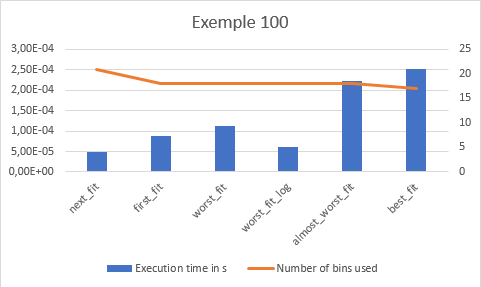
\includegraphics{exemple100.png}
\end{center}
\caption{Exemple 100}
\end{figure}
\begin{figure}
\begin{center}

exemple100

Tableau de comparaison des deux meilleurs algorithmes

\begin{tabular}{|l|c|r|}
  \hline
  Algorithme & Temps d'exécution en s & Boîtes utilisées \\
  \hline
  first\_fit & 8,70E-05 & 18 \\
  best\_fit & 25,3E-05  & 17 \\
  \hline
\end{tabular}




\subsection{Exemple capacité 500}
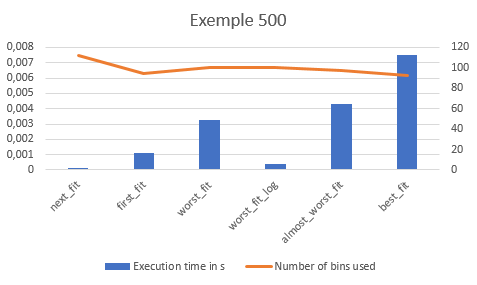
\includegraphics{exemple500.png}
\end{center}
\caption{Exemple 500}
\end{figure}
\begin{figure}
\begin{center}


exemple500

Tableau de comparaison des deux meilleurs algorithmes

\begin{tabular}{|l|c|r|}
  \hline
  Algorithme & Temps d'exécution en s & Boîtes utilisées \\
  \hline
  first\_fit & 1,09E-03 & 94 \\
  best\_fit & 7,49E-03  & 93 \\
  \hline
\end{tabular}


\subsection{Exemple capacité 1000}
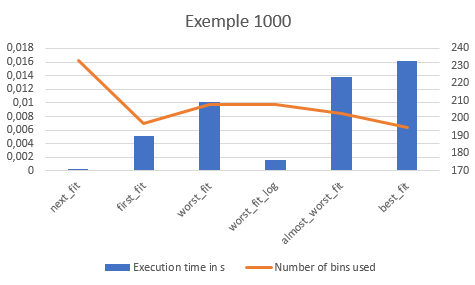
\includegraphics{exemple1000.png}
\end{center}
\caption{Exemple 1000}
\end{figure}
\begin{figure}
\begin{center}


exemple 1000

Tableau de comparaison des deux meilleurs algorithmes

\begin{tabular}{|l|c|r|}
  \hline
  Algorithme & Temps d'exécution en s & Boîtes utilisées \\
  \hline
  first\_fit & 5,13E-03 & 197 \\
  best\_fit & 16,15E-03  & 195 \\
  \hline
\end{tabular}


\subsection{Exemple proposé}
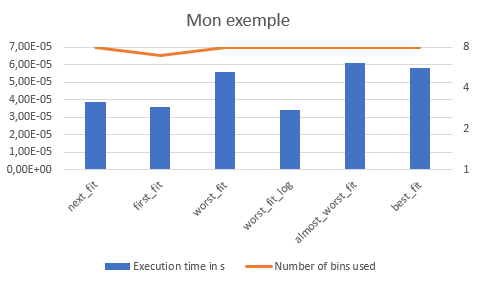
\includegraphics{monexemple.png}
\end{center}
\caption{Mon exemple}
\end{figure}


MonExemple


Tableau de comparaison des deux meilleurs algorithmes

\begin{tabular}{|l|c|r|}
  \hline
  Algorithme & Temps d'exécution en s & Boîtes utilisées \\
  \hline
  first\_fit & 3,60E-05  & 7 \\
  best\_fit & 5,80E-05  & 8 \\
  \hline
\end{tabular}


first_fit est le seul algorithme à avoir utilisé 7 boîtes contre 8 pour les autres algorithmes.


\subsection{Conclusion}

Les deux meilleurs algorithmes pour les 4 exemples cités précédemment sont best_fit et first_fit,
best_fit réussi toujours à mieux optimiser le packing des objets que first_fit mais dans un temps un peu plus elevé.
La différence de ces temps restant assez négligeable pour les cas 100, 500 et 1000, il conviendrait mieux d'utiliser best_fit pour un packing optimal
Néanmoins comme le montre monexample il y a des exceptions, dans ce cas les boites sont de capacité 524,
les objets sont triés dans l'ordre décroissant ce qui avantage first_fit et leur somme vaut exactement un multiple de 524
Nous avons essayé de réitérer cet exemple avec quelques capacités différentes nous avons pas réussi à obtenir la même chose.
Ce cas étant un cas assez peu courant à priori, nous aurons plutôt tendance à utiliser best_fit.

source du monexample
https://people.sc.fsu.edu/~jburkardt/datasets/bin_packing/bin_packing.html



\end{document}